\documentclass{beamer}
\usetheme{metropolis}           % Use metropolis theme

\usepackage[T2A]{fontenc}
\usepackage[utf8]{inputenc}
\usepackage[english, main=russian]{babel}

\usepackage{listingsutf8}
\usepackage[ruled]{algorithm}
\usepackage{algorithmicx}
\usepackage[noend]{algpseudocode}
\usepackage{amsmath}
\usepackage{caption} 
\usepackage{graphicx}
\usepackage{subcaption}
\usepackage{float}

\floatname{algorithm}{Листинг}
\renewcommand{\algorithmname}{Листинг}

\title{Визуализация графа связей пользователей социальной сети}
\date{\today}
\author{Киселев Кирилл}
\author[me]{Выполнил: Киселев Кирилл ИУ9-51Б\\[1mm]Руководитель: Каганов Ю.Т.}
% \thanks
% \institute{МГТУ им. Н.Э. Баумана}
\begin{document}
\maketitle

\begin{frame}{Цели и задачи}
  \metroset{block=fill}
	\begin{alertblock}{Цель}
		Реализовать приложение позволяющее визуализировать данные о связях пользователей социальной сети в виде графа.
	\end{alertblock}
	\begin{alertblock}{Задачи}
    
		\begin{itemize}
			\item Сформулировать критерии качества визуализации графа;
			\item Изучить способы визуализции графов;
			\item Реализовать несколько алгоритмов визуализации графов;
			\item Сравнить реализованное решение с существущими;
		\end{itemize}
	\end{alertblock}
\end{frame}

\begin{frame}{Критерии качества визуализации}

	\begin{itemize}
		\item Минимимальность пересечений ребер;
		\item Равномерность распределение вершин;
		\item Однородность длин ребер;
		\item Наличие симметрии.
	\end{itemize}
\end{frame}

\begin{frame}{Силовые алгоритмы}

	\alert{Силовые алгоритмы} визуализации графов оперируют основными принципами \textbf{сил} и \textbf{энергии} в физическом смысле, чтобы достичь оптимального распределения узлов и рёбер в графе.

  \metroset{block=fill}
	\begin{alertblock}{Основные этапы работы}
		\begin{enumerate}
			\item Инициализация
			\item Определение сил
			\item Обновление координат
			\item Итерация
		\end{enumerate}
	\end{alertblock}



\end{frame}

\begin{frame}{Алгоритм Идеса}
	\begin{algorithm}[H]
		\floatname{algorithm}{MegaAlgorithm}
		\caption{Алгоритм Идеса}
		\begin{algorithmic}[1]
			{\ttfamily \small{
					\Function{$f_{spring}$}{$p_u, p_v$}
					\State $r \gets c_{spring}\log{\frac{\|p_v - p_u \|}{l}}  \cdot \overrightarrow{p_u p_v}$

					\Return $r$
					\EndFunction


					\Function{$f_{rep}$}{$p_u, p_v$}
					\State $r \gets \frac{c_{rep}}{\|p_v - p_u \|} \cdot \overrightarrow{p_u p_v}  $

					\Return $r$
					\EndFunction


					\Function{Eades}{$G = (V, E)$, $p = (p_{v})_{v \in V}$, $k \in \mathbb{N}$}
					\State $t \gets 1$
					\While{$t \leq K$}

					\For{$u \in V$}
					\State $F_{u}(t) \gets \sum_{v:\{u,v\} \notin E}{f_{rep}(u, v)} + \sum_{v:\{u,v\} \in E}{f_{spring}(u, v)}$


					\EndFor
					\For{$u \in V$}
					\State $p_u \gets p_u + \delta \cdot F_u(t)$
					\EndFor

					\State $t \gets t + 1$
					\EndWhile
					\Return $p$
					\EndFunction

				}}

		\end{algorithmic}
	\end{algorithm}
\end{frame}
\begin{frame}{Алгоритм Фрюхтермана-Рейнгольда}
	\begin{algorithm}[H]
		\caption{Основной алгоритм}
		\begin{algorithmic}[1]

			{\ttfamily \small{
					\Function{FruchtermanReingold}{$G = (V, E)$, $p = (p_{v})_{v \in V}$, $k \in \mathbb{N}$}
          \State $t \gets initialize_t(G)$
					\While{$k \leq K$}

					\For{$u \in V$}
					\State $F_{u}(k) \gets \sum_{v \in V}{f_{rep}(u, v)} + \sum_{v:\{u,v\} \in E}{f_{attr}(u, v)}$


					\EndFor
					\For{$u \in V$}
					\State $p_u \gets p_u + \delta(t) \cdot F_u(k)$
					\EndFor

					\State $t \gets cool(t)$
					\State $k \gets k + 1$
					\EndWhile
					\Return $p$
					\EndFunction
				}}

		\end{algorithmic}
	\end{algorithm}
\end{frame}
\begin{frame}{Алгоритм Фрюхтермана-Рейнгольда}
	\begin{algorithm}[H]
		\caption{Нахождение сил притяжения и отталкивания}
		\begin{algorithmic}[1]

			\Function{$f_{rep}$}{$p_u, p_v$}
			\State $r \gets \frac{l^2}{\|p_v - p_u \|}  \cdot \overrightarrow{p_v p_u}  $

			\Return $r$
			\EndFunction


			\Function{$f_{attr}$}{$p_u, p_v$}
			\State $r \gets \frac{\|p_v - p_u \|^2}{l} \cdot \overrightarrow{p_u p_v}  $

			\Return $r$
			\EndFunction

		\end{algorithmic}
	\end{algorithm}
\end{frame}
\begin{frame}{Алгоритм Камады-Кавай}
	\begin{algorithm}[H]
		\caption{Алгоритм Камада-Кавай}
		\begin{algorithmic}[1]

			{\ttfamily \small{
					\Function{KamadaKawai}{$G = (V, E)$, $\varepsilon$, $p = (p_{v})_{v \in V}$}
					\State $d \gets FloydWarshall(G)$

					\State $initialize(l_{i, j})$
					\State $initialize(k_{i, j})$

					\State \While{$max_i \Delta_i$ > $\varepsilon$}

					\State $\Delta_m \gets max_i \Delta_i$
					\While{$\Delta_m$ > $\varepsilon$}
					\State $\text{Вычислить} \ \delta x, \delta y \ \text{решив следующую систему}$

					\State $ \frac{\partial^2 E}{\partial x^{2}_m}(x_m, y_m)\delta x + \frac{\partial^2 E}{\partial x_m \partial y_m}(x_m, y_m)\delta y = -\frac{\partial E}{\partial x_m}(x_m, y_m) $
					\State $ \frac{\partial^2 E}{\partial y_m \partial x_m}(x_m, y_m)\delta x + \frac{\partial^2 E}{\partial y^{2}_m}(x_m, y_m)\delta y = -\frac{\partial E}{\partial y_m}(x_m, y_m) $

					\State $p_m.x = p_m.x + \delta x$
					\State $p_m.y = p_m.y + \delta y$
					\EndWhile
					\EndWhile

					\State \Return $p$
					\EndFunction
				}}

		\end{algorithmic}
	\end{algorithm}

\end{frame}


\begin{frame}{Архитектура приложения }

	\begin{figure}
		\begin{minipage}{0.5\textwidth}
			\begin{alertblock}{Этапы работы приложения}
				\begin{enumerate}
					\item Сбор данных социлаьной сети
					\item Преобразование полученных данных в структуры ЯП
					\item Обработка данных силовым алгоритмом
					\item Отображение графа
				\end{enumerate}
			\end{alertblock}
		\end{minipage}
		\hfill
		\begin{minipage}{0.47\textwidth}
			\centering
			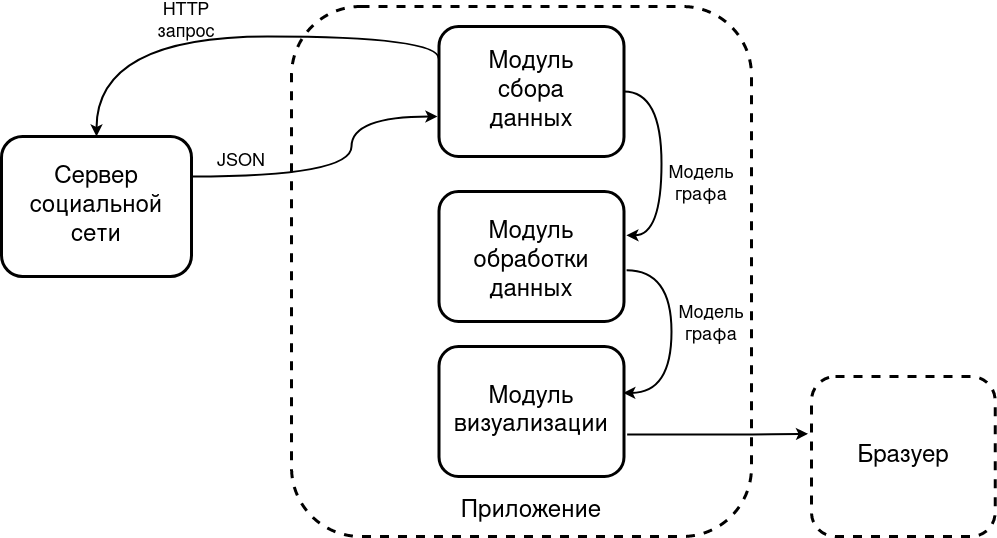
\includegraphics[width=\linewidth]{./imgs/app_scheme.png}
			\caption{Схема работы приложения}
		\end{minipage}
	\end{figure}

\end{frame}
\begin{frame}{Пример работы программы}

	\begin{figure}[H]
		\centering
		\begin{subfigure}[b]{0.48\textwidth}
			% \begin{minipage}[t]{.25\textwidth}
			\centering
			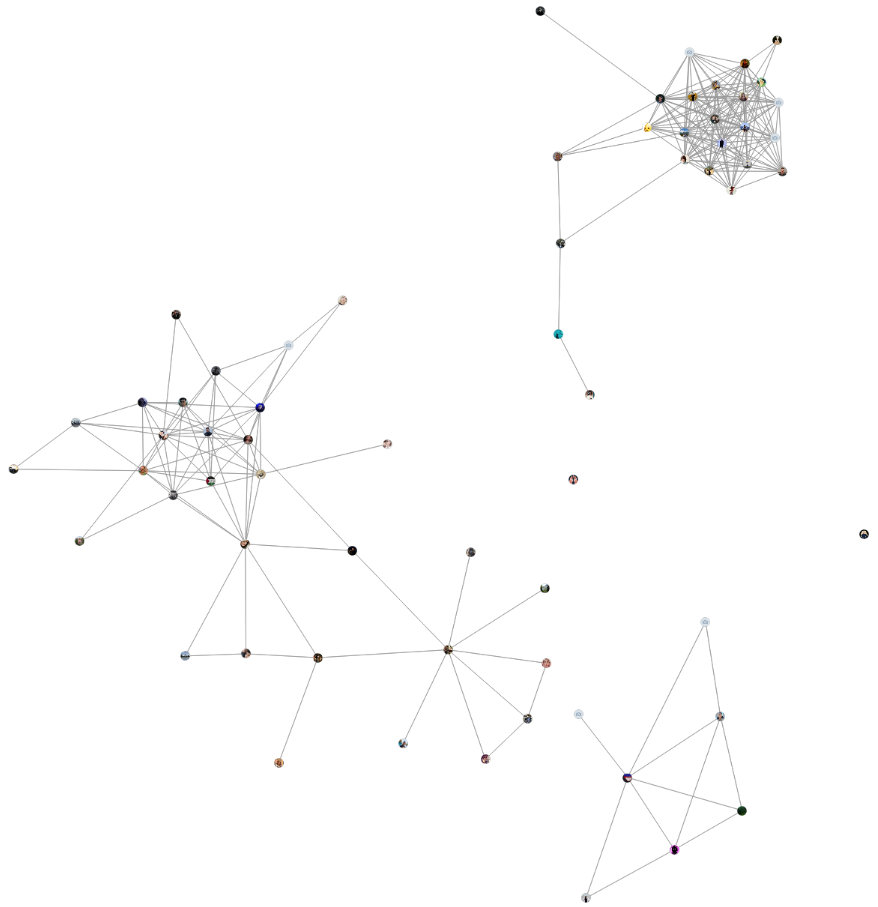
\includegraphics[width=\linewidth]{./imgs/fr.png}
			% \captionsetup{font=small}
			\caption*{алгоритм Фрюхтермана-Рейнгольда.}
		\end{subfigure}
		% \noindent
		\begin{subfigure}[b]{0.50\textwidth}
			\centering
			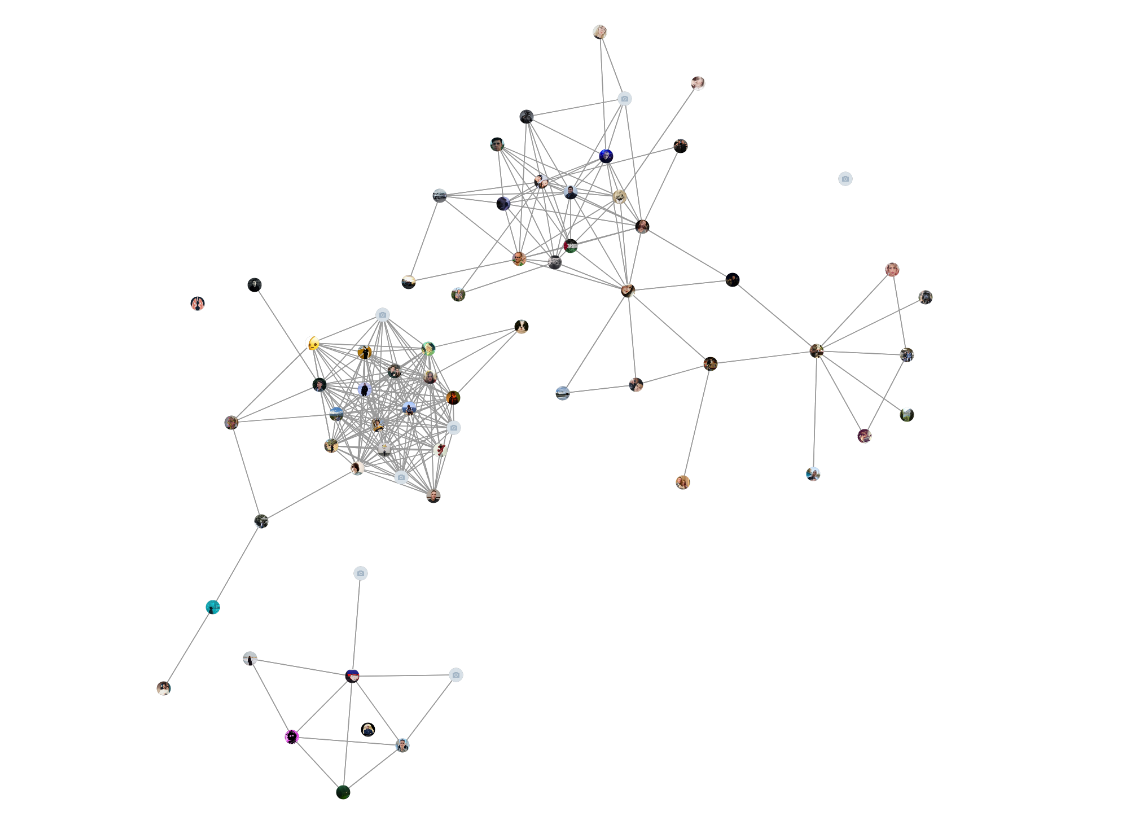
\includegraphics[width=\linewidth]{./imgs/kk.png}
			\captionsetup{font=small}
			\caption*{алгоритм Камады-Кавай.}
		\end{subfigure}
		\caption{Результат работы программы}
	\end{figure}


\end{frame}

\begin{frame}{Сравнение с Graphviz}
	\begin{figure}[H]
		\centering
		\begin{minipage}[t]{.32\textwidth}
			\centering
			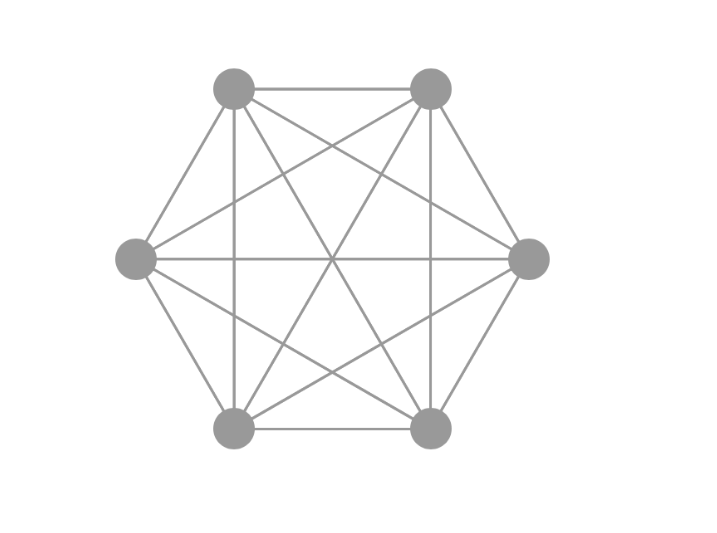
\includegraphics[width=\linewidth]{./imgs/fg_k6.png}
			\caption*{алгоритм Фрюхтермана-Рейнгольда.}
		\end{minipage}
		\noindent
		\begin{minipage}[t]{.32\textwidth}
			\centering
			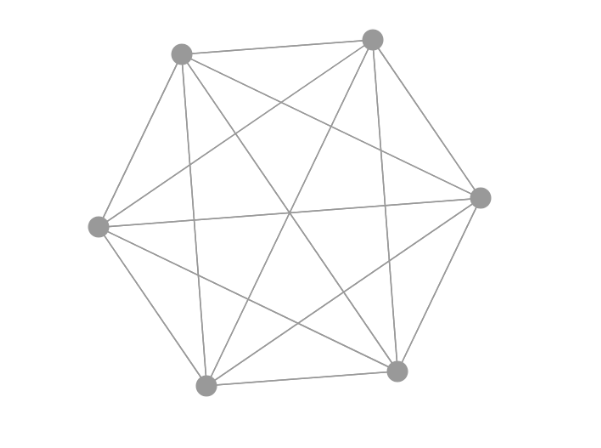
\includegraphics[width=\linewidth]{./imgs/kk_k6.png}
			\caption*{алгоритм Камады-Кавай.}
		\end{minipage}
		\begin{minipage}[t]{.32\textwidth}
			\centering
			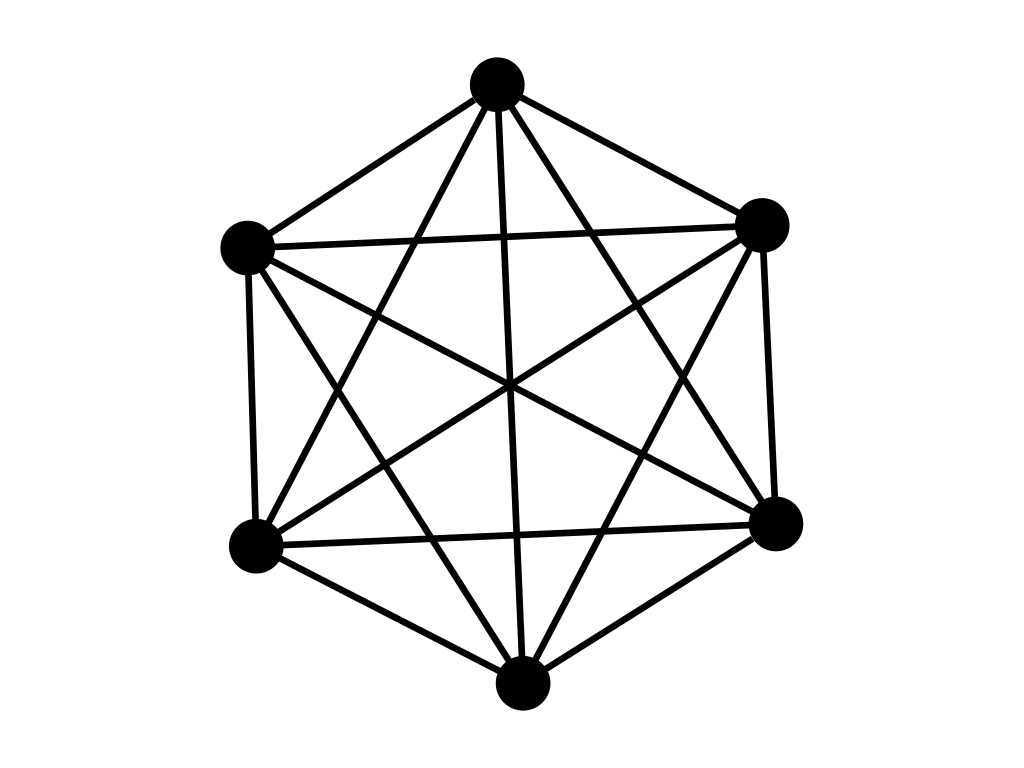
\includegraphics[width=\linewidth]{./imgs/k6_gv.png}
			\caption*{Graphviz.}
		\end{minipage}
		\caption{Результат работы программы на полном графе.}
	\end{figure}
\end{frame}



\begin{frame}{Сравнение с Graphviz}
	\begin{figure}[H]
		\centering
		\begin{minipage}[t]{.32\textwidth}
			\centering
			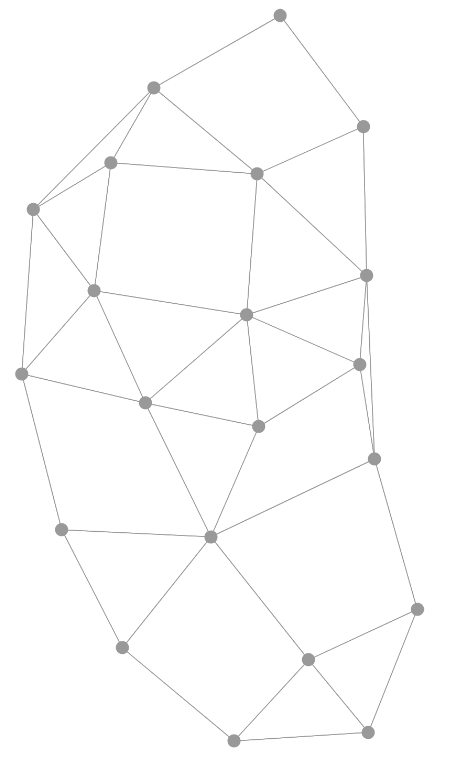
\includegraphics[width=0.75\linewidth]{./imgs/fg_small_dense.png}
			\caption*{алгоритм Фрюхтермана-Рейнгольда}
		\end{minipage}
		\noindent
		\begin{minipage}[t]{.32\textwidth}
			\centering
			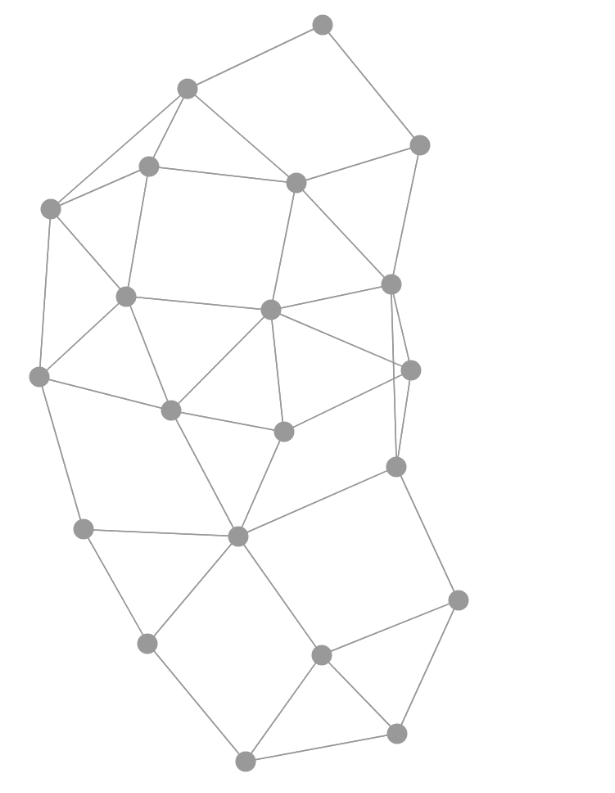
\includegraphics[width=0.9\linewidth]{./imgs/kk_small_dense.png}
			\caption*{алгоритм Камады-Кавай}
		\end{minipage}
		\begin{minipage}[t]{.32\textwidth}
			\centering
			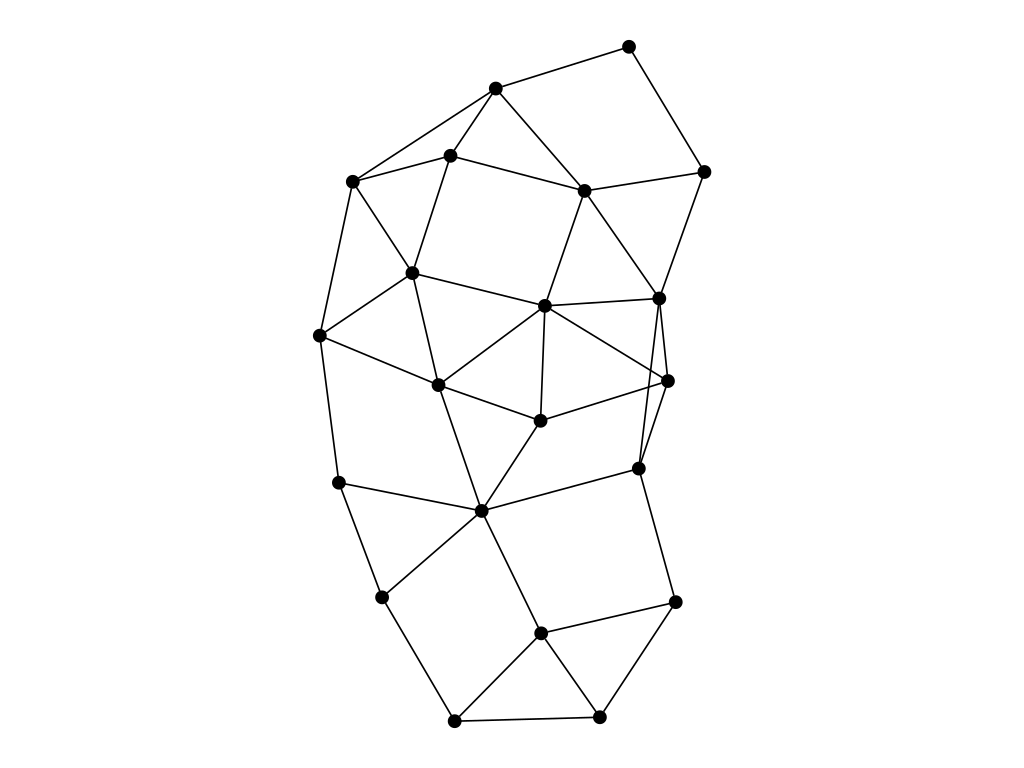
\includegraphics[width=1.4\linewidth]{./imgs/small_dense_gv.png}
			\caption*{Graphviz}
		\end{minipage}
		\caption{Результат работы программы на небольшом плотном графе.}
	\end{figure}
\end{frame}

\begin{frame}{Сравнение с Graphviz}
	\begin{figure}[H]
		\centering
		\begin{minipage}[t]{.32\textwidth}
			\centering
			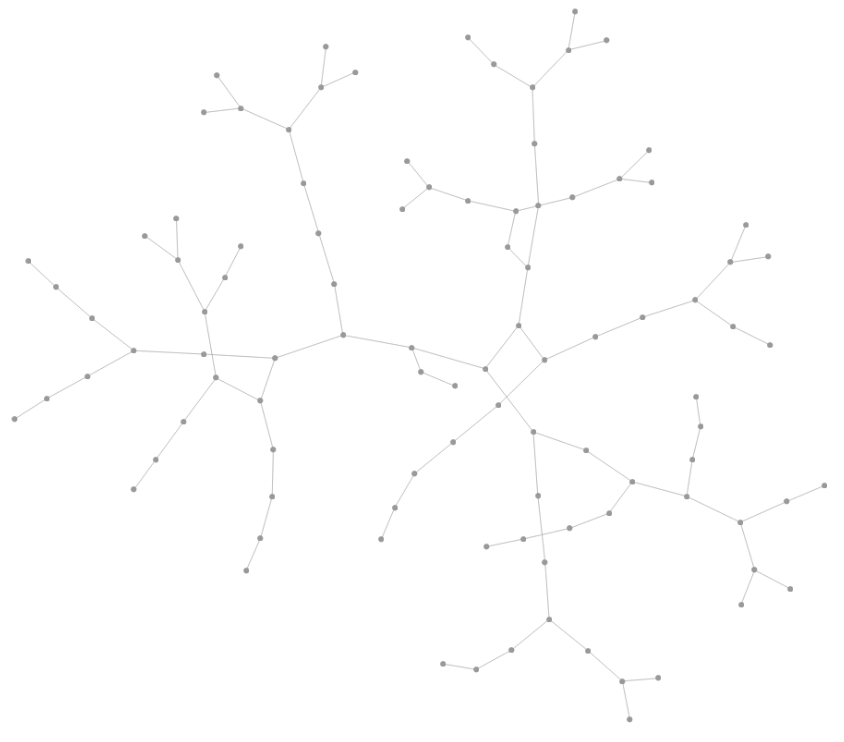
\includegraphics[width=\linewidth]{./imgs/fr_btree.png}
			\caption*{алгоритм Фрюхтермана-Рейнгольда}
		\end{minipage}
		\noindent
		\begin{minipage}[t]{.32\textwidth}
			\centering
			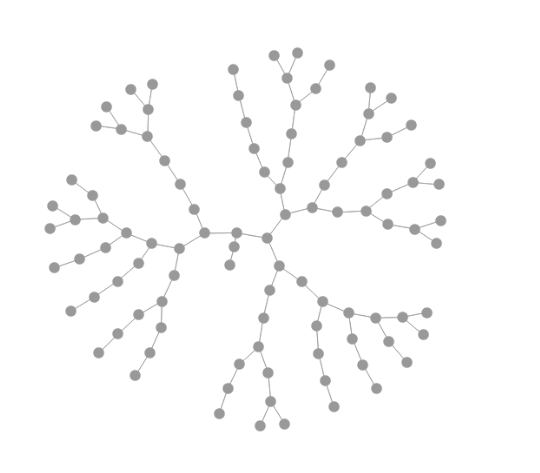
\includegraphics[width=\linewidth]{./imgs/kk_btree.png}
			\caption*{алгоритм Камады-Кавай}
		\end{minipage}
		\begin{minipage}[t]{.32\textwidth}
			\centering
			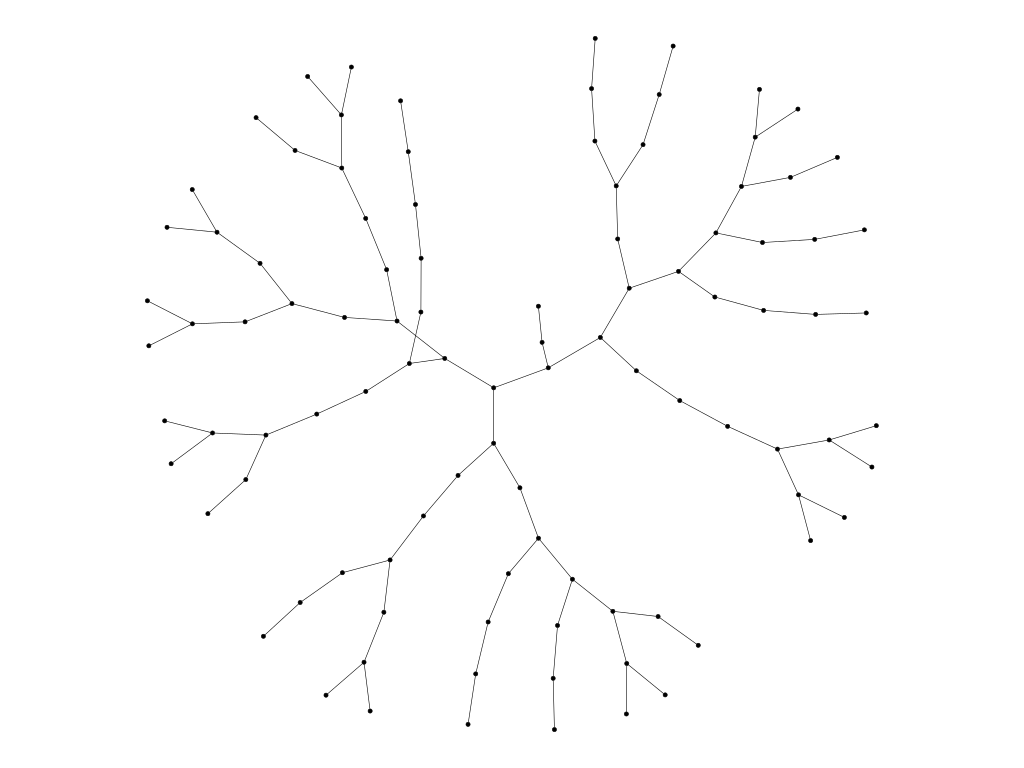
\includegraphics[width=\linewidth]{./imgs/bin_tree_gv.png}
			\caption*{Graphviz.}
		\end{minipage}
		\caption{Результат работы программы на бинарном дереве.}
	\end{figure}
\end{frame}

\begin{frame}{Сравнение с Graphviz}
	\begin{figure}[H]
		\centering
		\begin{minipage}[t]{.32\textwidth}
			\centering
			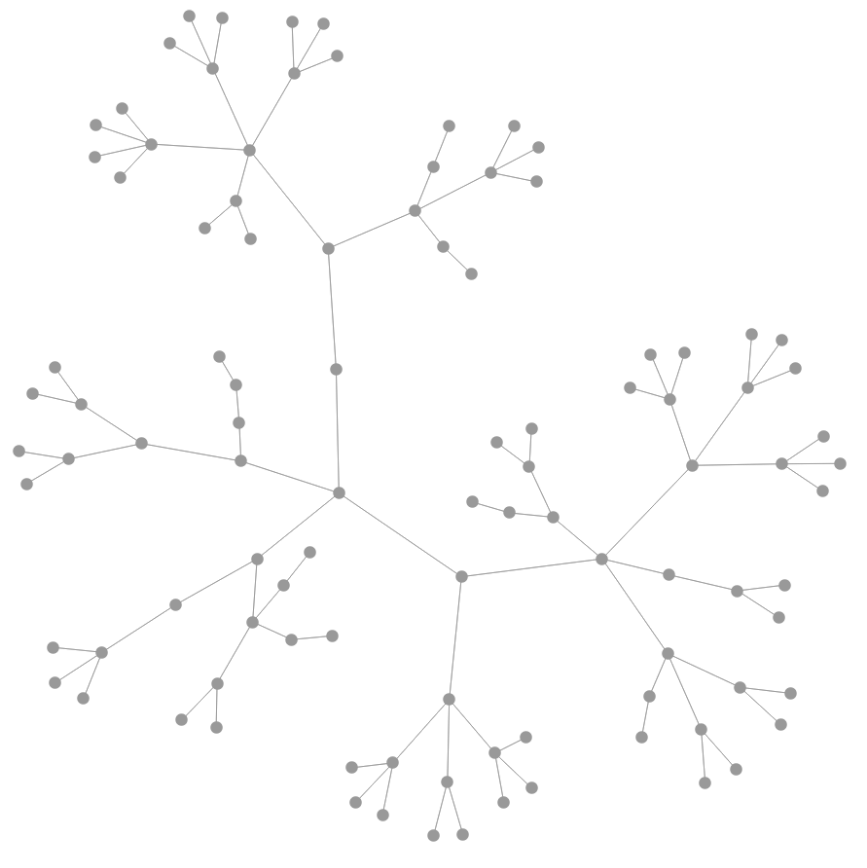
\includegraphics[width=\linewidth]{./imgs/fr_quad_tree.png}
			\caption*{алгоритм Фрюхтермана-Рейнгольда}
		\end{minipage}
		\noindent
		\begin{minipage}[t]{.32\textwidth}
			\centering
			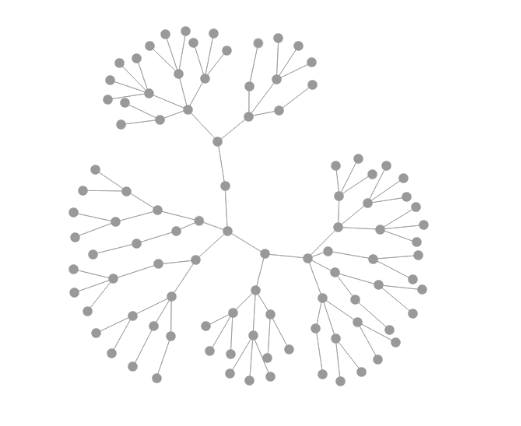
\includegraphics[width=\linewidth]{./imgs/kk_quad_tree.png}
			\caption*{алгоритм Камады-Кавай}
		\end{minipage}
		\begin{minipage}[t]{.32\textwidth}
			\centering
			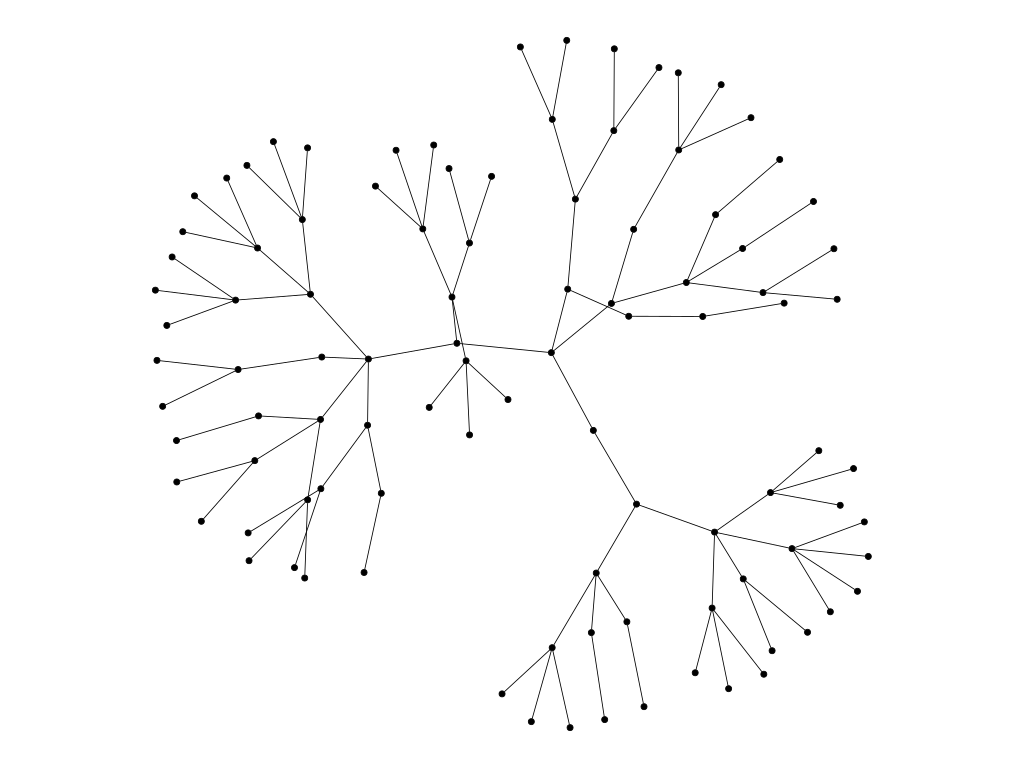
\includegraphics[width=\linewidth]{./imgs/quad_tree_gv.png}
			\caption*{Graphviz}
		\end{minipage}
		\caption{Результат работы программы на k-арном дереве, при k=4.}
	\end{figure}
\end{frame}

\begin{frame}{Заключение}
  \begin{alertblock}{Возможные улучшения}
  \begin{itemize}
    \item Покрытие кода модульными тестами; 
    \item Написание модулей сбора данных для большего числа соц. сетей; 
    \item Графическое выделение сообществ пользователей; 
  \end{itemize}
  \end{alertblock}
\end{frame}

\begin{frame}{Заключение}
  В ходе разработки были получены следующие навыки:
    \begin{itemize}
      \item Разработка силовых алгоритмов и их применение к задаче визуализации связей пользователей соц. сетей;
      \item Разработка на языке TypeScript;
      \item Использование библиотеки Cytoscape.js для визуализации графовых данных;
    \end{itemize}
\end{frame}



\end{document}
